%!TEX TS-program = pdflatex
%!TEX root = i3det-top.tex
%!TEX encoding = UTF-8 Unicode

\section{Introduction}
\label{sec:intro}

% \subsection{IceCube Science}
In the six decades following the experimental
discovery of the neutrino by Cowan and Reines, detectors have been realized
that have steadily progressed toward the goal of neutrino
astronomy.  Early developments in the field included the first detections of
atmospheric neutrinos in deep underground telescopes \cite{Achar,Witwatersrand} and
radiochemical detection of the flux of neutrinos from
nuclear fusion in the Sun \cite{Homestake}. A couple dozen neutrino
events were detected from supernova 1987A
\cite{SK1987A,IMB1987A,BUST1987A}, providing the first glimpse of neutrinos
from outside the solar system.  Advanced
atmospheric and solar neutrino observatories provided definitive
evidence of neutrino mass and constrained neutrino mixing
parameters \cite{SK,SNO}.  The study of neutrinos emanating from astrophysical
processes has both informed and sometimes surprised the fields of
astrophysics and particle physics. 

Neutrinos, because of their weak interaction and electrically neutral character, are useful probes of high
energy phenomena in the Universe. Unlike photons, detecting their origins in astrophysical
acceleration sites would unambiguously indicate hadronic acceleration and
provide identification of the origins of cosmic rays. Neutrinos arrive 
undeflected and unscattered upon detection and thus point back to their
originators, providing
a clear view of the physics deep within shrouded and compact sources. At
the most extreme energies, they are the only particles that can reach 
us from sources at cosmological distances. Notwithstanding the events seen from SN1987A, a remarkable but
extremely rare class of phenomena, the detection of neutrinos originating in
astrophysical processes outside our solar system requires detector facilities of
extreme dimensions to detect the faint fluxes of these weakly-interacting
particles. 

Progress toward large-scale neutrino observatories using arrays of
photomultiplier tubes (PMTs) in water or ice was achieved through the efforts of
DUMAND \cite{DUMAND}, Baikal \cite{Baikal}, AMANDA \cite{AMANDA:detector}, and
ANTARES \cite{ANTARES}.  These experiments provided key measurements of the
high-energy atmospheric neutrino spectrum, constrained optimistic models of
astrophysical neutrino production, and demonstrated the feasibility of the
technique. However, the detection of astrophysical neutrinos proved
elusive, suggesting that a kilometer-scale array was required to achieve the necessary sensitivity.  

The IceCube Neutrino Observatory is a cubic-kilometer neutrino detector
built into the ice at the South Pole. Construction was completed
on December 18, 2010 and commissioning was completed in 2011.  Its primary scientific objective has been the discovery of
astrophysical neutrinos, which was achieved in 2013 \cite{IC3:evidence}, and the 
identification and characterization of their sources.  Other science
objectives include indirect detection of dark matter, searches for other exotic particles,
studies of neutrino oscillation physics, and detection of the neutrino burst
from a Galactic core-collapse supernova.  A multi-messenger collaboration
with optical, X-ray, gamma-ray, radio, and gravitational wave observatories
provides multiple windows onto the potential neutrino sources.  A key to
the success of these initiatives is the reliability and performance of the
IceCube instrumentation, as well as the flexibility and stability of the
online software systems.  

\subsection{A Functional Description of the IceCube Observatory}

In order to detect neutrinos, IceCube exploits the fact that charged
particles resulting from neutrino interaction move through the
ice faster than the phase velocity of light in ice, and therefore emit Cherenkov photons. An enormous detection volume
is required due to the small interaction cross-section of neutrinos
and the extremely low fluxes expected at Earth from astrophysical
objects. The ice cap at the South Pole is about three~km thick and is
a suitable
operational site, since it not only offers a large quantity of interaction
material but also a medium with excellent optical qualities.  With a
Cherenkov photon yield of $\mathcal{O}(\num{E5})$ visible photons per
\SI{}{\giga\electronvolt} of secondary particle shower energy, the long
optical attenuation length of South Pole ice, and large-area PMTs, it is possible to instrument cubic kilometers of
ice with a rather sparse spacing of detectors. IceCube is located at the Amundsen-Scott
South Pole Station, which offers the logistical support
required for the construction and operation of the observatory.

The basic detection unit in IceCube is the
digital optical module (DOM), covered in detail in Sec.~\ref{sec:dom}.
Encapsulated in a \SI{0.5}{''}-thick glass pressure sphere 
to withstand the extreme pressure in the deep ice, the main components of a DOM
are a \SI{10}{''} PMT, embedded high-voltage generation, an LED Flasher 
Board, and a Main Board containing the analog and digital processing circuitry
for PMT pulses.  The transmission of the digital data is controlled by an FPGA
and embedded processor hosted on the Main Board. Detector calibration
is described in Sec.~\ref{sec:dom_calibration}. The digitized data are sent to a
central computing facility at the surface via a cable system described in
Sec.~\ref{sec:cable}.  Aspects of detector deployment and ice drilling are
covered in Sec.~\ref{sec:drill-deploy}. An overview of the data flow as well as
its readout, processing and filtering are presented in
Sec.~\ref{sect:online}, along with data handling, monitoring, and operational performance of
the observatory. The IceCube Neutrino Observatory consists of a subsurface
``in-ice'' array of DOMs, including a the more densely instrumented
DeepCore sub-array, and the IceTop surface array.  The entire detector
uses the same DOM design and associated surface readout. A schematic layout
of the Observatory is shown in Fig.~\ref{fig:array}. 

\begin{figure}[!h]
 \centering
 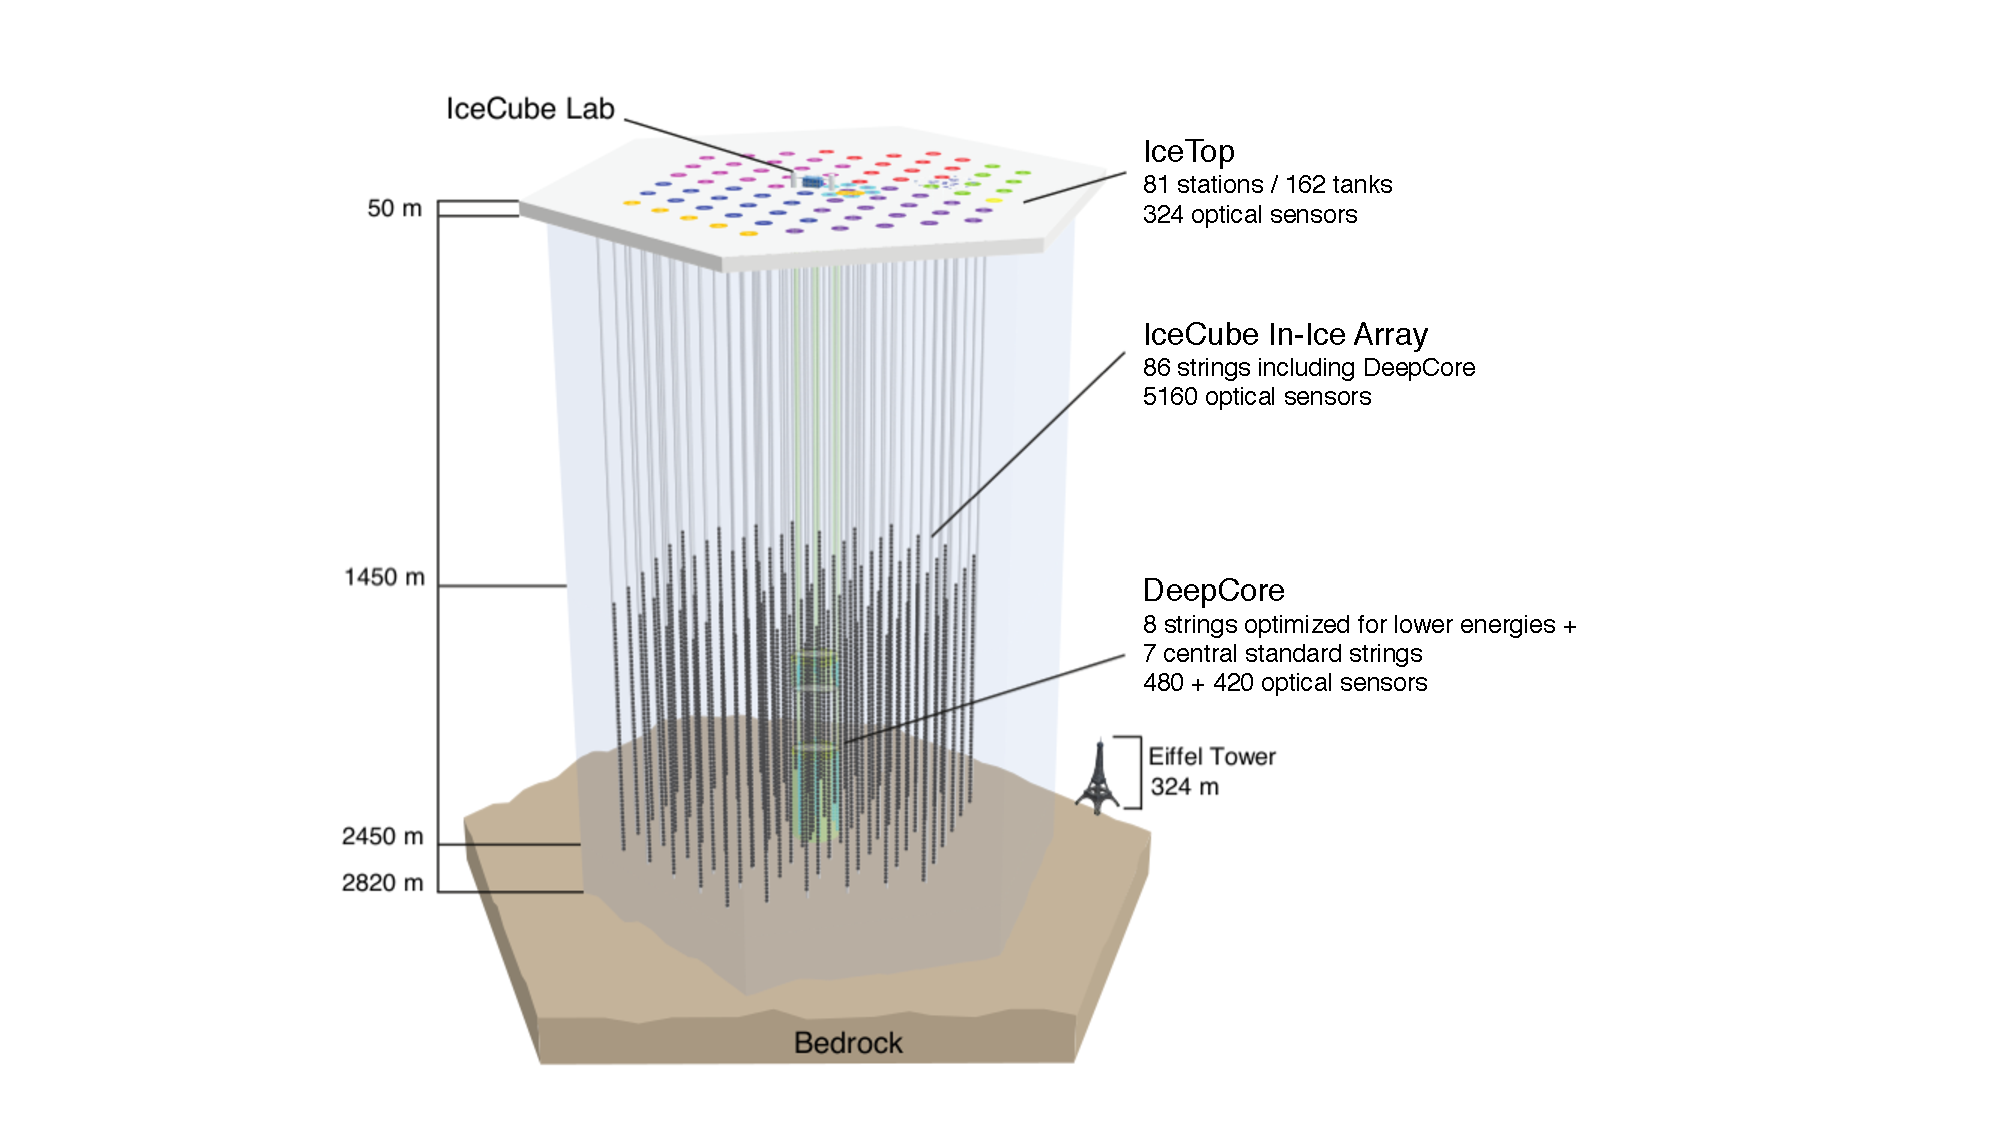
\includegraphics[width=\textwidth]{graphics/intro/ArrayWSeasonsLabels_crop.pdf}
 \caption{The IceCube Neutrino Observatory with the in-ice array, its sub-array DeepCore, and
   the cosmic-ray air shower array IceTop. The different string/station colors
   represent different deployment seasons.}
 \label{fig:array}
\end{figure}

\subsubsection{IceCube In-Ice Array}

In order to detect the Cherenkov photons emitted by charged particles
traversing the ice, \num{5160} DOMs are deployed between \SI{1450}{\meter}
and \SI{2450} {\meter} below the surface of the ice on \num{86} vertical
strings, with each string consisting of \num{60} DOMs deployed along a
single cable containing twisted copper-wire pairs. The 
primary in-ice array consists of \num{78} strings with a vertical
separation of the DOMs of \SI{17}{\meter}.  The strings are
deployed on a hexagonal grid with \SI{125}{\meter} horizontal spacing
that includes an instrumented volume of of one cubic kilometer of ice.  This design was chosen in
order to meet the primary science requirement of detecting astrophysical
neutrinos in the energy range of $\mathcal{O}(\SI{}{\tera\electronvolt})$--
$\mathcal{O}(\SI{}{PeV})$.  % The observation of these neutrinos was achieved
% by searching for events that start inside the volume of IceCube and deposit
% more than \SI{30}{\tera\electronvolt} of energy \cite{IC3:evidence}. 

Two different event topologies form the standard signatures of neutrinos in
IceCube.  Track-like events originate from a charged current interaction of
a high-energy muon neutrino with a nucleus, producing a hadronic shower at
the vertex and an outgoing muon that emits a Cherenkov cone along its
track.  The angular reconstruction of such a muon track and hence the
incident neutrino direction can reach a resolution better than
$\SI{1}{\degree}$, confirmed by analysis of the Moon's shadow
in cosmic rays \cite{IC3:moon}. Energy loss of muons above the minimum-ionizing regime, typically $ \sim
\SI{1}{\tera\electronvolt}$ in ice, is dominated by stochastic
processes resulting in large fluctuations in the amount of energy deposited
for different muons of the same energy.  A second class of events are
electromagnetic or hadronic showers from interactions of all neutrino
flavors, resulting in a more spherical light generation in the detector.
Since the total light output of such a shower is directly proportional to its energy, and
the showers are often well-contained in the detector, the neutrino energy
reconstruction for such events is much more precise than for track-like
events. The average deposited energy resolution for both event types
combined is about $\SI{15}{\%}$ \cite{IC3:ereco}. 

\subsubsection{DeepCore}

A subset of in-ice DOMs is deployed deeper than \SI{1750}{\meter} with a denser instrumented volume and
correspondingly lower energy threshold. This
sub-array, DeepCore \cite{ICECUBE:DC}, consists of eight specialized and
closely-spaced strings of sensors in the center of the array, along with
the seven central standard IceCube strings. The inter-string spacing
in DeepCore varies from \SI{41}{\meter} to \SI{105}{\meter}, with an
average spacing of \SI{72}{\meter}.

The eight specialized DeepCore strings have a DOM-to-DOM spacing of
\SI{7}{\meter} for the bottom 50 DOMs, deployed at depths of
\SI{2100}{\meter} to \SI{2450}{\meter}.  The remaining 10 DOMs are
deployed at depths shallower than \SI{2000}{\meter} with a spacing of
\SI{10}{\meter} to form a veto cap, allowing better rejection of downgoing
atmospheric muons.  Depths from \SI{2000}{\meter} to \SI{2100}{\meter}
are not instrumented, as the optical scattering and absorption is
significantly increased in this region of the ice (the ``dust layer''~\cite{Aartsen:2013rt}).

Six of the specialized DeepCore strings are fully instrumented with
DOMs using PMTs with \SI{35}{\%} higher quantum efficiency than the
standard IceCube modules. The remaining two specialized strings are
equipped with a mixture of standard and higher quantum efficiency DOMs. The denser geometry and increased efficiency
result in a lower energy threshold of about
\SI{10}{\giga\electronvolt}, compared to about
\SI{100}{\giga\electronvolt} for most IceCube analyses. The DeepCore design
is optimized for the detection of atmospheric neutrinos with energies
from \SI{10}{\giga\electronvolt} to \SI{100}{\giga\electronvolt}
\cite{ICECUBE:DC}. 

\subsubsection{IceTop}

The cosmic ray air shower array IceTop \cite{ICECUBE:IceTop} consists
of \num{162} Cherenkov tanks filled with clear ice and arranged in
\num{81} pairs on the
surface, using approximately the same grid on which the in-ice
array is deployed. A denser infill array is formed by the eight
stations in the center of IceTop, corresponding to the denser
inter-string spacing
in DeepCore. Each tank is \SI{1}{\meter} high, with a \SI{1.82}{\meter} inner diameter and is
filled with ice to a height of \SI{0.90}{\meter}.  The two tanks at each surface station are separated from
each other by \SI{10}{\meter}. Each tank contains two standard IceCube
DOMs, one ``high-gain'' DOM operated at a PMT gain of $5 \times 10^{6}$, and one
``low-gain'' DOM operated at a gain of $10^{5}$, to increase the dynamic range for air shower detection. Air showers initiated in the atmosphere by cosmic rays are typically
spread over a number of stations. The light generated in the tanks by the
shower particles (electrons, photons, muons and hadrons) is a measure of
the energy deposition of these particles in the tanks. IceTop is sensitive to
primary cosmic rays in the energy range of \SI{}{PeV} to \SI{}{EeV}
with an energy resolution of \SI{25}{\%} at \SI{2}{PeV}, improving to
\SI{12}{\%} above \SI{10}{PeV} \cite{IT:measurement}. For the infill
array the energy threshold is lowered to about \SI{100}{TeV}. The energy range of IceCube as a cosmic-ray detector fully covers the ``knee'' region of the spectrum and extends to the energies where a transition from galactic cosmic rays to a population of extra-galactic
particles may occur. The IceTop array has additionally been used to study high-pT muons, PeV gamma rays and transient events, such as the radiation effects of solar flares. It also serves as a partial veto for the detection of downward-going neutrinos with IceCube.  




